\apendice{Especificación de diseño}

\section{Introducción}
En esta parte del anexo definiremos como se han resuelto los objetivos expuestos anteriormente.
\section{Diseño de datos}
El proyecto cuenta con las siguientes entidades:
\begin{itemize}
	\item \textbf{Homogeneous Ensemble}: Es la encargada de llama a los distintos algoritmos que hemos realizado, todos tienen unos parámetros en común que serán los que tiene esta clase abstracta.
	\item \textbf{Disturbing Neighbors}: Este algoritmo lo usamos para aumentar la diversidad de los clasificadores base. El método crea características nuevas que se agregarán al conjunto de datos del clasificador base. Dichas características se calculan con el clasificador Nearest Neighbour(NN), construido a partir de unas instancias seleccionadas al azar. Para probar la eficacia utilizamos árboles de decisión como clasificador base.
	\item \textbf{Random Oracles}: Es un ensemble, en el cual, cada clasificador del cojunto se reemplaza por un miniensemble de un par de subclasificadores con un oráculo para elegir entre ellos.
	\item \textbf{Rotation Forest}: Es un ensemble, este método genera conjuntos de clasificadores basados en la extracción de características. Crea un conjunto de entrenamiento para un clasificador base, este conjunto se divide al azar en subconjuntos K y PCA se aplica a cada subconjunto. Las rotaciones del eje K tienen lugar para formas las nuevas características para un clasificador base. La idea es mejorar la precisión y diversidad dentro del conjunto. La diversidad se basa en la extracción de características para cada clasificador base.
\end{itemize}


\subsection{Diagrama de clases general}\label{diagram-general}
\begin{figure}
\centering
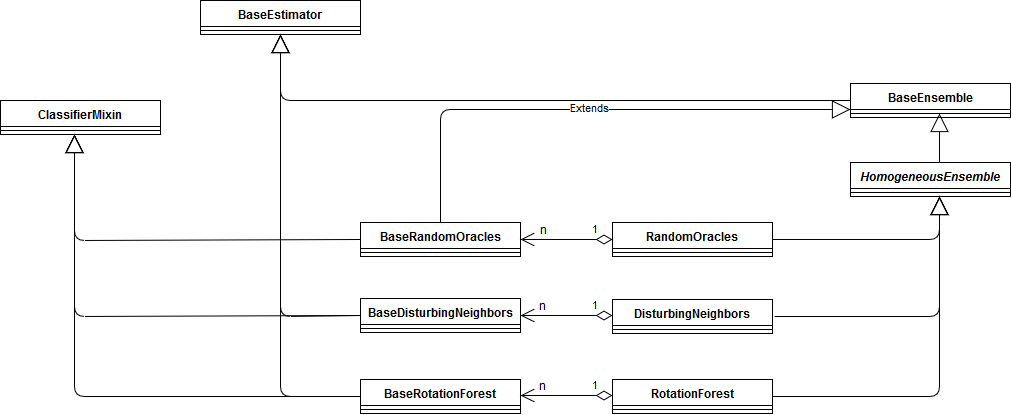
\includegraphics[width=0.95\textwidth]{DiagramGeneral}
\caption{Diagrama de clases general}
\label{fig:DiagramGeneral}
\end{figure}

\subsection{Diagrama de clases implementadas}\label{diagram-implement}
\begin{figure}
\centering
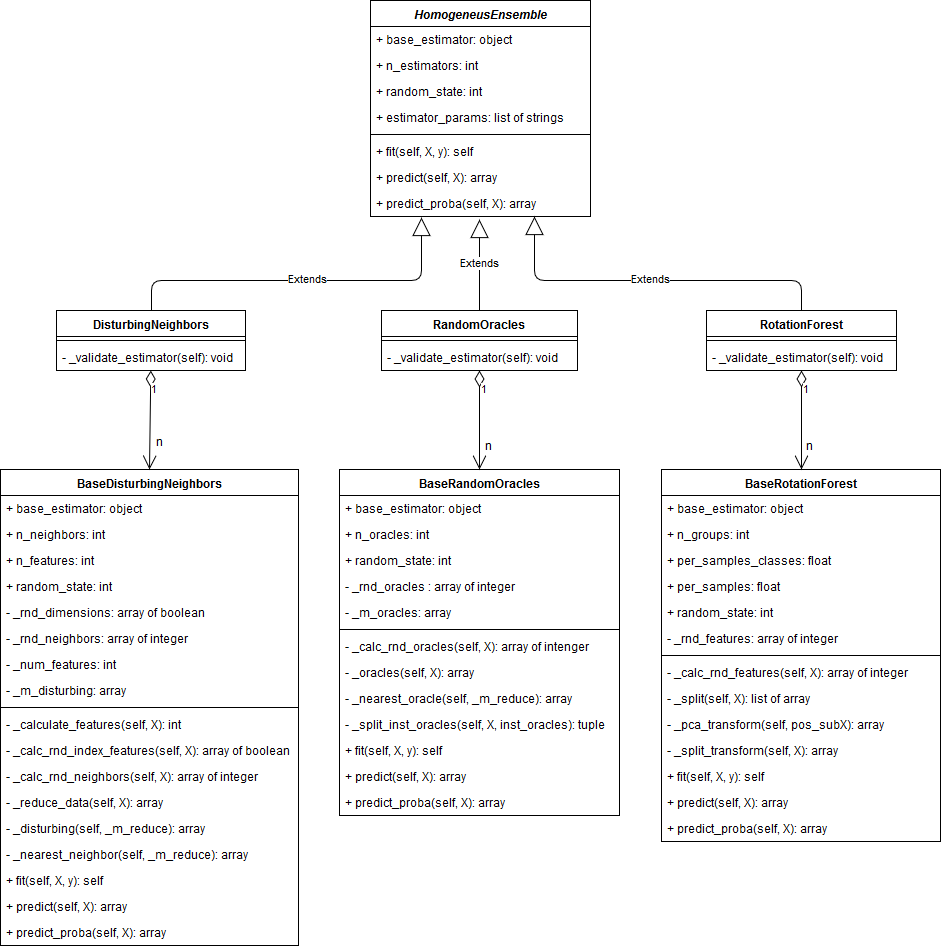
\includegraphics[width=0.95\textwidth]{DiagramImplement}
\caption{Diagrama de clases implementadas}
\label{fig:DiagramImplement}
\end{figure}

\subsection{Diagrama de secuencias}\label{diagrama-secuencias}
Se ha realizado un diagrama de secuencias de como seria un ejemplo de ejecución del ensemble Disturbing Neighbors.
\begin{figure}
\centering
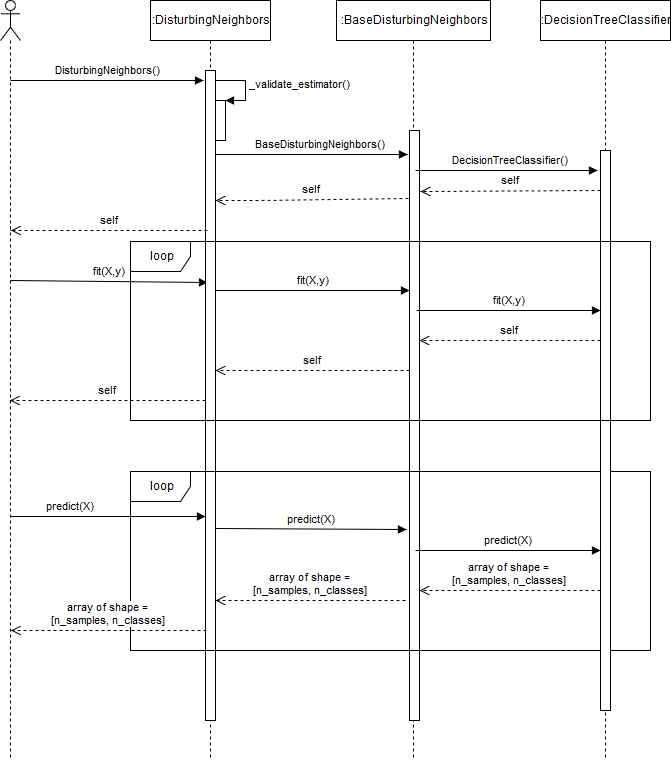
\includegraphics[width=0.95\textwidth]{DiagramSequence}
\caption{Diagrama de secuencias}
\label{fig:DiagramSequence}
\end{figure}

\section{Diseño procedimental}

\section{Diseño arquitectónico}


